%% Lab 02 implementation paper. ACM acmart (acmsmall). pdfLaTeX + BibTeX (Overleaf default).
\documentclass[acmsmall,nonacm]{acmart}

\usepackage{booktabs}
\usepackage{tabularx}
\newcolumntype{L}[1]{>{\raggedright\arraybackslash}p{#1}}
\newcolumntype{Y}{>{\raggedright\arraybackslash}X}
\setcopyright{none}
\settopmatter{printacmref=false}

\begin{document}

\title{Judging a Reference by How It Looks: How Much Does Surface Form Reveal About Fabricated Citations?}

\author{Farigh A. Sabri}
\affiliation{%
  \institution{IIITA}
  \city{Prayagraj}
  \country{India}}

\begin{abstract}
My earlier review asked whether a more elaborate citation format raises readers' trust in a reference, found no study that isolates format, and rested part of its argument on the premise that format says nothing about whether a reference is real. Here I test that premise computationally: how well can a detector that sees only the surface of a reference, and never looks it up, tell fabricated citations from real ones? I reproduce a published surface-feature control from the HALLMARK benchmark (exactly, at the commit that reported it), extend it with three groups of reader-visible cues, and compare it with a character n-gram model, a completeness rule and a majority baseline, under a protocol fixed before any of my models were scored. On HALLMARK's held-out test split the best surface model reaches AUROC 0.797 (95\% CI 0.765--0.825), within the range of eight released zero-shot LLM verifiers (0.59--0.78). Most of this signal sits in the easiest error types, and part of it comes from artefacts of how the benchmark generated its fakes. Completeness itself carries almost none (AUROC 0.515). On 341 ChatGPT citations human-coded by Walters and Wilder, where real and fabricated references share one generator and one format, models trained on HALLMARK fall to chance (0.51--0.55), and even models trained on that set reach only 0.679 under topic-grouped cross-validation, against 0.957 for a database lookup tool. The appearance of a reference, in short, says little about whether it exists once benchmark artefacts are removed.
\end{abstract}

\begin{CCSXML}
<ccs2012>
<concept><concept_id>10002951.10003227.10003392</concept_id><concept_desc>Information systems~Digital libraries and archives</concept_desc><concept_significance>500</concept_significance></concept>
<concept><concept_id>10010147.10010257</concept_id><concept_desc>Computing methodologies~Machine learning</concept_desc><concept_significance>300</concept_significance></concept>
<concept><concept_id>10003120.10003121</concept_id><concept_desc>Human-centered computing~Human computer interaction (HCI)</concept_desc><concept_significance>100</concept_significance></concept>
</ccs2012>
\end{CCSXML}
\ccsdesc[500]{Information systems~Digital libraries and archives}
\ccsdesc[300]{Computing methodologies~Machine learning}
\ccsdesc[100]{Human-centered computing~Human computer interaction (HCI)}
\keywords{citation hallucination, fabricated references, surface features, benchmark artefacts, reproducibility, trust calibration}

\maketitle

%% =================================================================
\section{Introduction}

A reference list makes a promise: each entry points to something a reader could find. Most readers never check. They see author names, a year, a venue and perhaps a DOI, and they move on. In my literature review \cite{sabri2026review} I argued that this habit may rest on a shortcut. A reference that \emph{looks} complete may be read as one that \emph{is} sound, in the same way that other surface cues are read as signs of credibility \cite{metzger2013,newman2012}. The review separated five things that are easily confused: whether a citation is present, its surface format, whether the source exists, whether it supports the claim, and whether the reader verifies it. Its central question, whether a more elaborate format raises trust when existence and relevance are held constant, could not be answered from the literature. Part of its argument also rested on a premise it did not test at scale: that the format of a reference carries no information about whether the source exists. This paper tests that premise, the link between surface format and existence.

Two published results point in different directions. Walters and Wilder found that 55\% of GPT-3.5 references and 18\% of GPT-4 references in their sample were fabricated, yet the fabricated entries followed APA style as closely as the real ones \cite{walters2023}. Naser, on the other hand, reports that a classifier using only the text of a reference separated real from hallucinated citations with an AUC of 0.876 \cite{naser2026}. If Naser's result holds generally, a reader who judges by appearance is not entirely wrong. If Walters and Wilder's observation is the rule, appearance is close to useless.

Testing the human side of this needs participants and ethics approval, which a one-week lab cannot provide. This paper tests the side that can be measured with code: \emph{how much a reader who sees only the surface of a reference could know, at best}. I use detectors as stand-ins for an idealised reader who notices every visible cue but never opens a database. The paper asks three questions:

\begin{description}
  \item[RQ1] On a labelled benchmark, how well do surface-only detectors separate fabricated from real references, and for which kinds of error?
  \item[RQ2] Does that ability survive on references where real and fake come from the same generator and share one format?
  \item[RQ3] Which surface cues carry the signal, and how much is left once differences in formatting are removed?
\end{description}

The contribution is a controlled comparison, not a new detector. It reproduces a published baseline exactly, makes one isolated extension to it, tests it on an external human-coded set that removes the benchmark's main confound, and reports where the signal comes from, including where it comes from the benchmark rather than from the citations.

%% =================================================================
\section{Background}

\paragraph{Surface cues and trust.} Credibility research describes how people fall back on cheap cues (design quality, apparent thoroughness, endorsement) when checking is costly \cite{metzger2013}. Processing fluency adds that material which proves nothing can still raise belief \cite{newman2012}. Ding et al.\ showed experimentally that attaching citations to a chatbot answer raised trust even when the citations were irrelevant, and that checking a citation lowered it \cite{ding2025}. None of these studies asks whether the cue is \emph{diagnostic}. In Lee and See's terms, trust is well calibrated only if it tracks actual reliability \cite{leesee2004}.

\paragraph{How often models fabricate.} Fabrication rates depend strongly on model, topic and prompt \cite{walters2023,linardon2025,naser2026}. Fabricated references also appear in accepted papers at NeurIPS 2025, often combining several realistic details so that each one passes a different quick check \cite{ansari2026}.

\paragraph{Detection.} Most detectors look references up: they match fields against Crossref, OpenAlex or Semantic Scholar \cite{naser2026,shi2026citeaudit}. Others ask the model itself indirect questions and use the inconsistency of its answers \cite{agrawal2024}. HALLMARK \cite{reizinger2026hallmark,hallmarkrepo} is a benchmark of 2,525 labelled BibTeX entries across 14 hallucination types in three difficulty tiers. Its authors include a \emph{shortcut control}: a gradient-boosting classifier on 24 surface features, used to check whether some hallucination types can be detected without any verification. They found that it detects four ``real-paper'' types at a rate of 0.468 on dev and 0.388 on test, and they treat this as a benchmark limitation. That control is the baseline I reproduce and extend.

%% =================================================================
\section{Data}

\begin{table}[t]
\caption{Evaluation data. All files come from HALLMARK v1.2.4 at commit \texttt{c62d296}, checked against recorded SHA-256 sums.}
\label{tab:data}
\small
\begin{tabularx}{\textwidth}{@{}L{3.6cm}rrrY@{}}
\toprule
Set & Real & Fabricated & Total & Role and notes \\
\midrule
HALLMARK \texttt{dev\_public} & 504 & 615 & 1,119 & Training and threshold selection only \\
HALLMARK \texttt{test\_public} & 307 & 524 & 831 & Held out; 14 hallucination types, 3 tiers \\
Walters \& Wilder ChatGPT set & 172 & 169 & 341 & External; GPT-3.5/GPT-4 journal citations, human-coded; every entry has the same four fields; 40 topics \\
\bottomrule
\end{tabularx}
\end{table}

Table~\ref{tab:data} lists the data. In HALLMARK, real entries are scraped from DBLP, while most fabricated entries are generated by perturbing real ones, by prompting LLMs, or are collected from real incidents. This creates an obvious risk. A detector might learn the difference between ``scraped'' and ``generated'' formatting rather than between real and fake.

The external set addresses this. HALLMARK's maintainers converted the coded supplement of Walters and Wilder \cite{walters2023} into BibTeX: 341 journal citations written by ChatGPT, each coded by hand as real or fabricated. Real and fake share a generator. They also share a format: every entry has exactly author, title, journal and year. If surface form reveals fabrication in general, it should do so here too. Leakage checks found no shared keys between dev and test, one shared title (a fabricated entry) out of 831, and no overlap between the external set and HALLMARK.

A detector may read only the entry type and its fields. The loader removes the label, hallucination type, tier, explanation, generation method, source and the benchmark's sub-test results before any feature is computed.

%% =================================================================
\section{Method}

\begin{figure}[t]
  \centering
  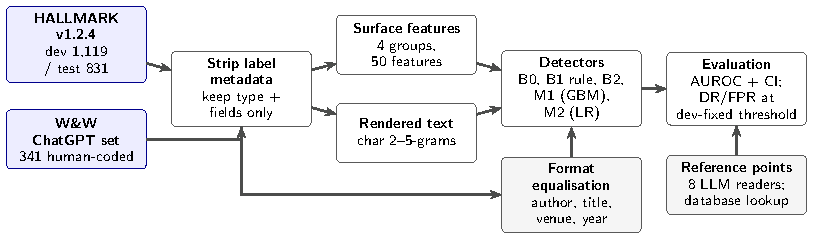
\includegraphics[width=\textwidth]{figures/pipeline.pdf}
  \caption{Study pipeline. Detectors never query a database. Reference points are released outputs of other tools, re-scored here, not rerun.}
  \label{fig:pipeline}
\end{figure}

\subsection{Detectors}
Figure~\ref{fig:pipeline} shows the pipeline. Five detectors are compared.
\textbf{B0}, a majority-class baseline, gives every entry the same score.
\textbf{B1}, a completeness rule, stands in for a reader who trusts references that look finished. It counts six visible components (author, title, year, venue, DOI or URL, pages or volume) and scores an entry as more suspicious the fewer it has.
\textbf{B2} is HALLMARK's shortcut control: gradient boosting with scikit-learn defaults \cite{pedregosa2011} on the authors' 24 surface features (field presence, string lengths, author count, entry type, year, arXiv DOI). I ported the feature function verbatim.
\textbf{M1} makes one change to B2: it adds three feature groups that a careful reader could check by eye. These are \emph{author style} (share of initials, surname lengths, duplicated surnames, non-ASCII names), \emph{title style} (capitalisation, digits, punctuation, word length, acronyms) and \emph{identifier consistency} (whether the DOI is well formed, DOI prefix length, whether a year embedded in a DOI or arXiv identifier agrees with the stated year, future years, the age of the reference). The learner and its settings are unchanged, giving 50 features in total.
\textbf{M2} works on the rendered text instead of features. It uses TF-IDF over character 2--5-grams of the reference as a reader would see it, followed by logistic regression. This is the closest analogue I could build to a string-only classifier.

\subsection{Protocol}
Everything below was fixed in a configuration file before any model of mine was scored on the test split or the external set. Models are fitted on \texttt{dev\_public} only. The decision threshold for each model and seed is the score at which five-fold cross-validated predictions on dev give a false-positive rate of 0.10. It is then applied unchanged to test and to the external set. The primary metric is AUROC (higher is better), reported with a stratified 1,000-sample bootstrap 95\% CI computed on the score averaged over five seeds (0--4). Secondary metrics are detection rate (DR, recall on fabricated references), false-positive rate (FPR) and MCC at the fixed threshold. On the external set I also train inside it, using stratified five-fold cross-validation grouped by literature-review topic so that citations from the same review never fall in both training and test folds.

I stated three hypotheses in advance. H1: surface detectors carry real signal on HALLMARK, concentrated in Tier~1. H2: models trained on HALLMARK do not transfer to the external set (AUROC $\le 0.60$ or a CI that includes 0.5). H3: even when trained on the external set, they stay below 0.80, well short of Naser's 0.876.

\subsection{Reference points}
Lookup-based tools could not be rerun, because Crossref, OpenAlex and Semantic Scholar were unreachable from my environment. I therefore re-scored released per-entry outputs against the current labels. These are eight zero-shot LLM verifiers on \texttt{test\_public}, which judge each entry without any bibliographic lookup (their logs list only the model endpoint), and bibtex-updater 1.4.0, a database-lookup tool, on the external set. They show what other approaches achieve. They are not baselines I validated.

%% =================================================================
\section{Baseline Validation}

\begin{table}[t]
\caption{Reproducing HALLMARK's surface-feature control (four real-paper types vs.\ real entries, five-fold CV, detection rate / FPR of gradient boosting).}
\label{tab:repro}
\small
\begin{tabularx}{\textwidth}{@{}YL{2.3cm}L{2.3cm}@{}}
\toprule
Condition & dev & test \\
\midrule
Reported in HALLMARK README & 0.468 / -- & 0.388 / -- \\
Original script at commit \texttt{fa0cc7b} (where the numbers were written) & 0.468 / 0.045 & 0.388 / 0.096 \\
Original script, parent of data commit \texttt{908a405} & 0.468 / 0.045 & 0.388 / 0.096 \\
Original script at \texttt{908a405} and at pinned v1.2.4 & 0.456 / 0.040 & 0.440 / 0.107 \\
My reimplementation on v1.2.4 & 0.456 / 0.040 & 0.440 / 0.107 \\
\bottomrule
\end{tabularx}
\end{table}

When I first ran HALLMARK's script on the current release, its numbers did not match the published ones (Table~\ref{tab:repro}). Running the unchanged script at three points in the repository history settled the question. The published numbers reproduce exactly up to the parent of commit \texttt{908a405}. That commit is the v1.2.4 ground-truth correction, which reverted 18 relabelled entries and restored 13 truncated fields, and it alone moves the numbers to 0.456 and 0.440. My reimplementation gives predictions identical to the original script, and my metric code matches HALLMARK's official metric functions on DR, FPR and AUROC to within $10^{-9}$. I treat the baseline as verified. All later B2 results use all 14 hallucination types and the train/test protocol above, so they are not directly comparable to this four-type check.

%% =================================================================
\section{Results}

\begin{table}[t]
\caption{Main results. AUROC is the mean of five seeds (seed SD $\le 0.005$ except grouped CV, $\le 0.027$); CI from the seed-averaged score. DR and FPR use the threshold fixed on dev (target FPR 0.10). Grouped CV has no fixed threshold.}
\label{tab:main}
\footnotesize
\setlength{\tabcolsep}{4pt}
\begin{tabularx}{\textwidth}{@{}L{2.5cm}YYYY@{}}
\toprule
 & HALLMARK test & HALLMARK test, & W\&W, transfer & W\&W, grouped CV \\
 & (full records) & format equalised & from HALLMARK & (trained on W\&W) \\
\midrule
B1 completeness rule & 0.515 [0.480, 0.550] & 0.512 [0.497, 0.527] & 0.500 & 0.500 \\
B2 HALLMARK GBM & 0.764 [0.732, 0.797] & 0.721 [0.686, 0.754] & 0.546 [0.489, 0.606] & 0.592 [0.537, 0.657] \\
M1 extended GBM & \textbf{0.797} [0.765, 0.825] & \textbf{0.748} [0.713, 0.778] & 0.549 [0.489, 0.608] & \textbf{0.679} [0.633, 0.744] \\
M2 char n-gram LR & 0.788 [0.755, 0.819] & 0.746 [0.713, 0.780] & 0.525 [0.459, 0.585] & 0.629 [0.569, 0.698] \\
\midrule
DR / FPR of M1 & 0.505 / 0.085 & 0.374 / 0.045 & 0.964 / 0.980 & -- \\
\midrule
Reference points & \multicolumn{2}{l}{8 LLM readers: 0.589--0.778} & \multicolumn{2}{l}{bibtex-updater (lookup): 0.957 [0.934, 0.977]} \\
\bottomrule
\end{tabularx}
\end{table}

\begin{figure}[t]
  \centering
  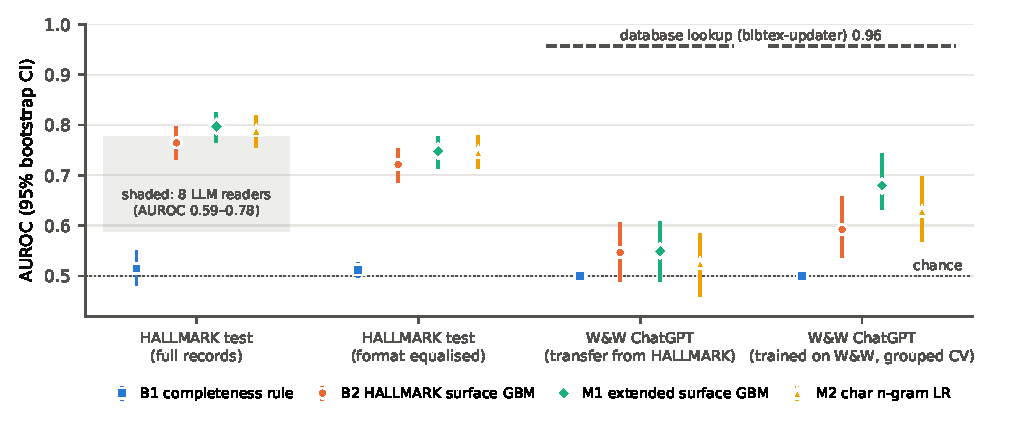
\includegraphics[width=\textwidth]{figures/fig_auroc_overview.pdf}
  \caption{AUROC with 95\% bootstrap CIs across the four evaluation conditions. The shaded band spans the eight released LLM readers on HALLMARK test; the dashed line is the database-lookup tool on the W\&W set. B0 sits at 0.5 throughout and is omitted.}
  \label{fig:overview}
\end{figure}

\subsection{RQ1: Surface form on the benchmark}
Table~\ref{tab:main} and Figure~\ref{fig:overview} summarise the results. On HALLMARK's held-out test split, all three learned surface detectors are clearly above chance. M1 reaches 0.797 [0.765, 0.825]. At the dev-fixed threshold it catches half of the fabricated entries (DR 0.505) and wrongly flags 8.5\% of the real ones. The single change from B2 to M1 (three added feature groups) improves AUROC by 0.033, with a paired bootstrap CI of [0.013, 0.054]. M1 and the text model M2 cannot be separated (difference 0.009, CI $-0.025$ to $0.043$). For comparison, the eight LLM verifiers that read the same entries without looking anything up range from 0.589 to 0.778. A cheap classifier on surface features is therefore as good as a large language model reading the citation, on this benchmark.

The completeness rule is the exception. With AUROC 0.515 [0.480, 0.550], how complete a reference looks tells almost nothing about whether it is real. Figure~\ref{fig:completeness} shows why. Real and fabricated entries in HALLMARK have nearly the same distribution of visible components, and in the W\&W set every entry has exactly four. In that set the rule cannot even rank the entries.

\begin{figure}[t]
  \centering
  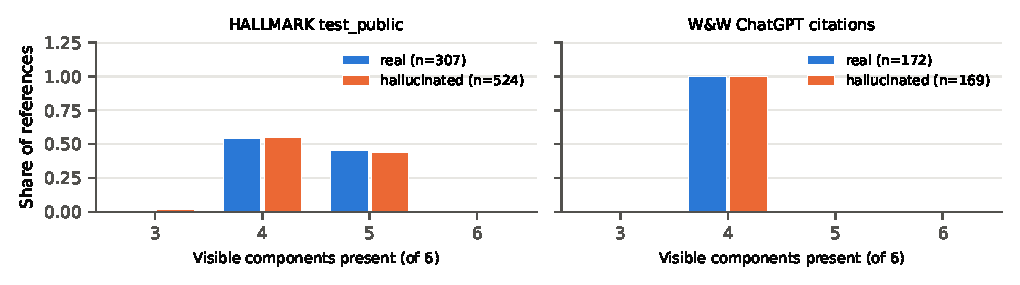
\includegraphics[width=\textwidth]{figures/fig_completeness.pdf}
  \caption{How many of six visible components each reference has, for real and fabricated entries. Completeness is almost identical between the classes, which is why the completeness rule (B1) performs at chance.}
  \label{fig:completeness}
\end{figure}

\begin{figure}[t]
  \centering
  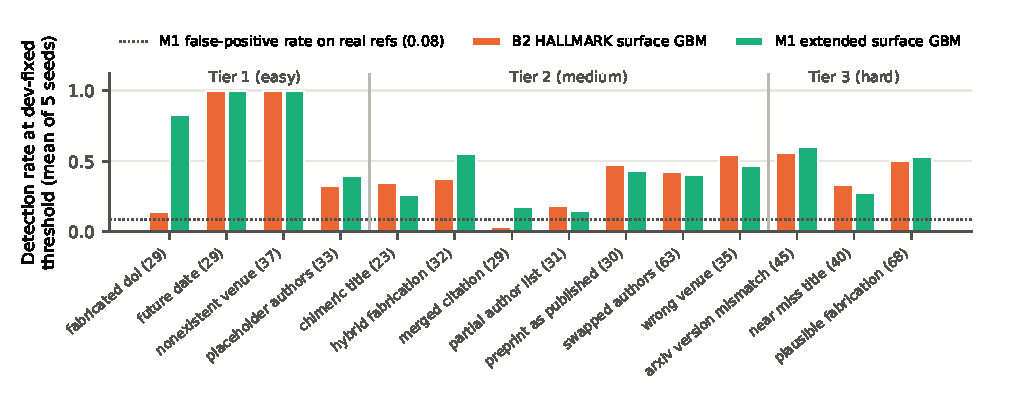
\includegraphics[width=\textwidth]{figures/fig_per_type.pdf}
  \caption{Detection rate by hallucination type on HALLMARK test at the dev-fixed threshold (mean of five seeds; counts in brackets). Dotted line: M1's false-positive rate on real references.}
  \label{fig:types}
\end{figure}

The signal is uneven across types (Figure~\ref{fig:types}). Types with a visible defect are caught almost perfectly: a future publication year (1.00) and a non-existent venue (1.00). Tier~1 as a whole is detected at 0.805 by M1. Tier~2 (0.360) and Tier~3 (0.482) are much harder. Merged citations (0.17) and partial author lists (0.15) are barely above the false-positive rate. H1 is supported: the signal is real and it sits mostly in the easy tier.

One gain needs a warning. M1 detects fabricated DOIs at 0.83, against 0.14 for B2. When I looked at the DOIs themselves, the fabricated ones in HALLMARK mostly use five-digit prefixes from unregistered ranges, such as \texttt{10.7777x} and \texttt{10.9999x}, while most real DOIs use four-digit publisher prefixes such as \texttt{10.1109}. M1's prefix-length feature picks this up. In an exploratory refit without the two prefix features, decided after seeing the per-type table, detection of fabricated DOIs falls to 0.31 and overall AUROC to 0.784. Most of that gain reflects how the benchmark generated its fakes, not something that would carry over to real fabrications.

\subsection{RQ2: When real and fake share a generator and a format}
On the W\&W ChatGPT citations, every model trained on HALLMARK falls to chance. AUROCs range from 0.511 to 0.549, and every CI includes 0.5, so H2 is supported. The fixed thresholds also fail. M1 flags 98\% of the real ChatGPT citations as fabricated, because these four-field journal entries look nothing like HALLMARK's real entries, which are scraped conference records. Whatever M1 learned on HALLMARK, much of it describes how that benchmark's real entries were collected.

Training on the W\&W set itself does better, but only modestly. Under topic-grouped cross-validation M1 reaches 0.679 [0.633, 0.744] and M2 0.629 [0.569, 0.698]. So there is some signal in how ChatGPT writes fabricated references, but it is far below Naser's reported 0.876, and H3 is supported. I do not read this as a refutation of Naser's result. His corpus, features and validation scheme differ, and his data are not available. A database lookup tool, by contrast, reaches 0.957 [0.934, 0.977] on the same 341 entries.

\subsection{RQ3: Which cues carry the signal}\label{sec:ablation}

\begin{figure}[t]
  \centering
  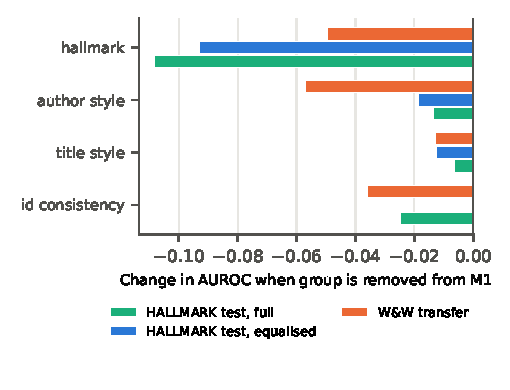
\includegraphics[width=0.62\textwidth]{figures/fig_ablation.pdf}
  \caption{Change in M1's AUROC when one feature group is removed (mean of five seeds).}
  \label{fig:ablation}
\end{figure}

Figure~\ref{fig:ablation} removes one feature group at a time from M1. On HALLMARK, the original HALLMARK features matter most: removing them costs 0.108 AUROC. Within them, the length of the venue string is the most important single feature. The benchmark authors flagged this same feature as leakage in their own control, and showed that it is not explained by how real entries were sampled. Identifier consistency adds 0.025 on full records and nothing once DOIs are removed, as it should. For transfer to W\&W, the author-style group matters most (removing it costs 0.057), although transfer stays near chance even with it included.

Format equalisation answers the second part of RQ3. When every entry is rewritten as author, title, venue and year, and the models are retrained, M1 drops from 0.797 to 0.748. About a sixth of M1's margin above chance (0.049 of 0.297) came from which fields were present. The rest comes from what is written in the remaining fields, so it is about wording, not formatting.

\subsection{Error analysis}
The fabricated references M1 trusts most are subtle ones: swapped authors, merged citations, near-miss and chimeric titles. In these the paper exists, or a plausible one could, and only a lookup would show the mismatch. Among its 25 most confident misses, 7 are swapped-author entries. Its most confident false positives tell another story. They are well-known real papers (\emph{Denoising Diffusion Probabilistic Models}, \emph{A Simple Framework for Contrastive Learning of Visual Representations}, \emph{Rethinking Attention with Performers}) cited with an arXiv DOI next to a conference name. That is ordinary citing practice, but it matches the pattern of one of HALLMARK's generated types (\texttt{arxiv\_version\_mismatch}). A reader who learned the benchmark's cues would grow suspicious of exactly the references that careful authors write.

%% =================================================================
\section{Discussion}

The review behind this paper asked whether a more elaborate citation format raises trust, and argued that such trust would be unearned if format says nothing about whether a reference exists. These experiments support that premise. For completeness, the cue the review focused on, the answer is clear: it carries no information. Completeness is equally common among real and fabricated references, and in the human-coded ChatGPT set it does not vary at all. Richer surface cues do carry signal on a synthetic benchmark. But that signal is concentrated in crude errors such as impossible years, invented venues and malformed identifiers, and part of it reflects how the benchmark was built. On authentic ChatGPT output it shrinks to a modest 0.68 at best and vanishes when a model trained elsewhere is applied. That is what one would expect if language models produce references that look right whether or not they exist \cite{walters2023}. It also fits the review's argument that format-based trust in such references cannot be calibrated \cite{leesee2004}, because format carries little information about existence.

There is also a methodological lesson for benchmarks. A surface classifier performing as well as large language models (0.80 against 0.59--0.78) is a warning about HALLMARK, not praise for the classifier. The benchmark's authors flagged part of this themselves. This study adds that the effect reaches beyond their four types, that it breaks down completely on external data, and that a feature which looks reasonable (DOI prefix length) can quietly learn the generator.

\paragraph{Limitations.} This study measures what a detector can extract from the surface of a reference. It does not measure what people notice or how much they trust it, which still requires the human experiment proposed in the review. The external set is small (341 entries) and limited to journal articles, because the conversion kept only that type, so its CIs are wide. HALLMARK's labels have been corrected several times, and further corrections may shift the numbers slightly. The reference-point tools were run by other people at earlier dates, and I could not verify their run conditions. Only CPU-scale models were tested. A large model fine-tuned on citation strings might extract more, although the transfer result suggests it would mostly extract more of the benchmark.

%% =================================================================
\section{Reproducibility and AI-Use Statement}
Code, configuration, logs, per-entry predictions and figure scripts are in the project repository. The reported results come from a run on my own laptop (Windows 11, Python 3.13.2). A run of the same code on Linux (Python 3.13.18) matched them to within 0.001 AUROC in every summary cell. Only the gradient-boosting models differ at all; this is most likely floating-point differences between platforms breaking near-ties in split selection. The text model and all reference points match exactly. \texttt{bash scripts/run\_all.sh} fetches the data at the pinned commit, verifies checksums, runs the tests, reproduces the baseline check and regenerates every table and figure in about five minutes on two CPU cores (Python 3.13, scikit-learn 1.9.1). Three protocol changes were made after results were seen, and all are logged: the majority baseline's score was fixed to a constant after a pooled-CV artefact, a mislabelled reference-point flag was corrected, and two analyses were added and labelled exploratory. An AI assistant (Claude, Anthropic) was used for code generation, debugging, analysis and drafting. The repository's \texttt{ai\_assistance\_log.md} records each significant use, the checks applied and the errors it made that were caught.

%% =================================================================
\section{Conclusion}
A reference's surface (whether it has a DOI, how long its venue string is, how its authors' names are written) separates fabricated from real citations on a synthetic benchmark about as well as an LLM reading it. Much of that comes from crude errors and from the benchmark itself. Completeness alone is uninformative. When real and fabricated references are written by the same model in the same format, surface cues carry little information, and a detector trained elsewhere is at chance. Checking a reference still means looking it up.

\begin{acks}
I thank the HALLMARK authors for releasing their data, code and per-entry outputs under an open licence, and Walters and Wilder for publishing their coded supplement.
\end{acks}

\bibliographystyle{ACM-Reference-Format}
\bibliography{references}

\end{document}
